\documentclass[compress, aspectratio=54]{beamer}
%\documentclass[notes=show]{beamer}
%\documentclass[xcolor=dvipsnames]{beamer}
\usepackage[export]{adjustbox}
\usepackage{sidecap}
\usepackage{subfig}
\usepackage{amssymb}
\usepackage{latexsym}
\usepackage{amsfonts}
\usepackage{amsmath}
\usepackage[absolute,overlay]{textpos}
\usepackage[english]{babel}
\usepackage[latin1]{inputenc}
\usepackage{subfig}
%\usepackage{times}
\usepackage[T1]{fontenc}
\usepackage{tabularx}
\newcolumntype{Y}{>{\small\raggedright\arraybackslash}X}
\usepackage{graphicx}
\usepackage{bigstrut}
\usepackage{bbm}
\usepackage{mathrsfs}
\usepackage{epsfig}
\usepackage{array}
%\usepackage{natbib}
\usepackage{hyperref}
\hypersetup{
    colorlinks=true,
    linkcolor=blue,
    filecolor=magenta,      
    urlcolor=cyan,
}
\usepackage{caption}
\usepackage{xcolor}

\mode<presentation> {
%\usetheme[left,width=1.7cm]{Berkeley}
%\usetheme{default}
\usetheme{Boadilla}
  \usecolortheme[RGB={103,102,204}]{structure}
%\usecolortheme{dove}
  \useoutertheme{infolines}
  \setbeamercovered{transparent}
 }

%\usepackage[utf8]{inputenc}

% Default fixed font does not support bold face
\DeclareFixedFont{\ttb}{T1}{txtt}{bx}{n}{12} % for bold
\DeclareFixedFont{\ttm}{T1}{txtt}{m}{n}{12}  % for normal

% Custom colors
\usepackage{color}
\definecolor{deepblue}{rgb}{0,0,0.5}
\definecolor{deepred}{rgb}{0.6,0,0}
\definecolor{deepgreen}{rgb}{0,0.5,0}

\usepackage{listings}

% Python style for highlighting
\newcommand\pythonstyle{\lstset{
language=Python,
basicstyle=\ttm,
otherkeywords={self},             % Add keywords here
keywordstyle=\ttb\color{deepblue},
emph={MyClass,__init__},          % Custom highlighting
emphstyle=\ttb\color{deepred},    % Custom highlighting style
stringstyle=\color{deepgreen},
frame=tb,                         % Any extra options here
showstringspaces=false            % 
}}


% Python environment
\lstnewenvironment{python}[1][]
{
\pythonstyle
\lstset{#1}
}
{}

% Python for external files
\newcommand\pythonexternal[2][]{{
\pythonstyle
\lstinputlisting[#1]{#2}}}

% Python for inline
\newcommand\pythoninline[1]{{\pythonstyle\lstinline!#1!}}
%\renewcommand{\familydefault}{cmss}
%\renewcommand{\mathrm}{\mathsf}
%\renewcommand{\textrm}{\textsf}
\usefonttheme{serif}
\newcommand{\X}{{\mathbf{X}}}
\newcommand{\x}{{\mathbf{x}}}
\newcommand{\E}{\mathsf{E}}
\newcommand{\V}{\mathsf{Var}}

\DeclareGraphicsExtensions{.jpg,.pdf,.mps,.png}

\setbeamercolor{bibliography entry title}{fg=black}
\setbeamercolor{bibliography entry author}{fg=black}
\setbeamercolor{subsection in toc}{fg=structure}
\setbeamercolor{palette primary}{bg=structure, fg=white}
%\setbeamercolor{palette secondary}{bg=structure, fg=black}
%\setbeamercolor{palette tertiary}{bg=structure, fg=black}
\setbeamercolor{caption name}{fg=black} \setbeamersize{text margin
left=.8cm} \setbeamersize{text margin right=1cm}
\hypersetup{linkbordercolor={1 0 0}} \setbeamertemplate{navigation
symbols}{} \setbeamertemplate{headline}[default]

\setbeamertemplate{enumerate items}[default]

\newcounter{transfct}
\newcounter{begbs}
\newcounter{endbs}


\title[Introduction to
K Means Clustering]{Machine Learning for Natural Language Processing}

\author[Arieda Mu\c co]{Arieda Mu\c co\footnote{Based on: Chapter 10 of Introduction to Statistical Learning By Gareth James, et al.}}
\institute[CEU]{Central European University}

\AtBeginSection[] {
  \begin{frame}<handout:0>
    \frametitle{TOC}
    \tableofcontents[currentsection]
  \end{frame}
}


\AtBeginSection[] {
  \begin{frame}<handout:0>
    \frametitle{TOC}
    \tableofcontents[currentsection]
  \end{frame}
}


\pgfdeclareimage[height=.7cm]{logo}{rgs2}
\logo{\pgfuseimage{logo}}
\begin{document}
\captionsetup[subfigure]{labelformat=empty}

\frame{\titlepage}

%%%%%%%%%%%%%%%%%%%%%%%%%%%%%%%%%%%%%%%%%%%


\begin{frame}

\frametitle{K Means Clustering}
\begin{itemize}
\item K Means Clustering is an unsupervised learning algorithm that
will attempt to group similar clusters together in your data.

\item So what does a typical clustering problem look like?
\begin{itemize}
\item Cluster Similar Documents
\item Cluster Customers based on Features
\item Market Segmentation
\item Identify similar physical groups
\end{itemize}
\end{itemize}

\end{frame}
%----------------------------------------------------------------------------%

\begin{frame}

\frametitle{K Means Clustering}
The overall goal is to divide data into distinct groups such
that observations within each group are similar

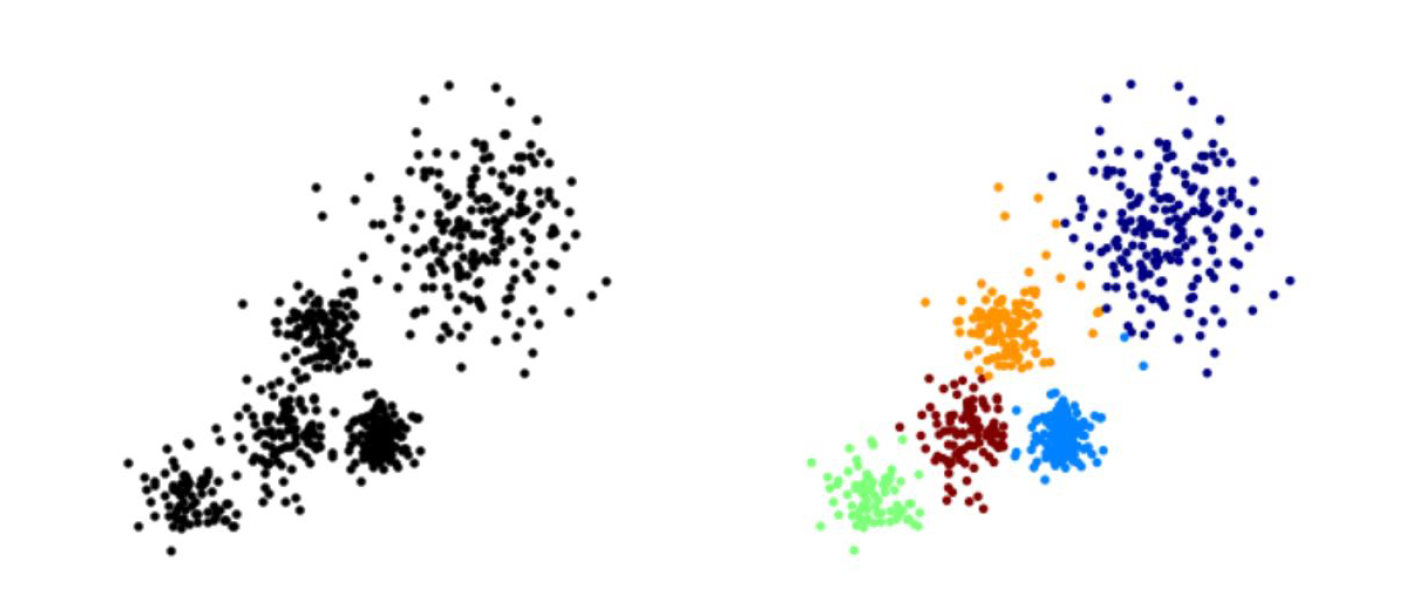
\includegraphics[width=0.85\linewidth ]{Figures/kmeans.png}


\end{frame}
%----------------------------------------------------------------------------%


%----------------------------------------------------------------------------%

%----------------------------------------------------------------------------%


\begin{frame}
\frametitle{K Means Clustering}
Choose a number of Clusters "K"
\begin{itemize}
\item Randomly assign each point to a cluster
\item Until clusters stop changing, repeat the following:
\begin{itemize}
\item For each cluster, compute the cluster centroid by
taking the mean vector of points in the cluster
\item Assign each data point to the cluster for which the
centroid is the closest

\end{itemize}
\end{itemize}

\end{frame}
%----------------------------------------------------------------------------%

\begin{frame}
\frametitle{K Means Clustering Algorithm}
\centering
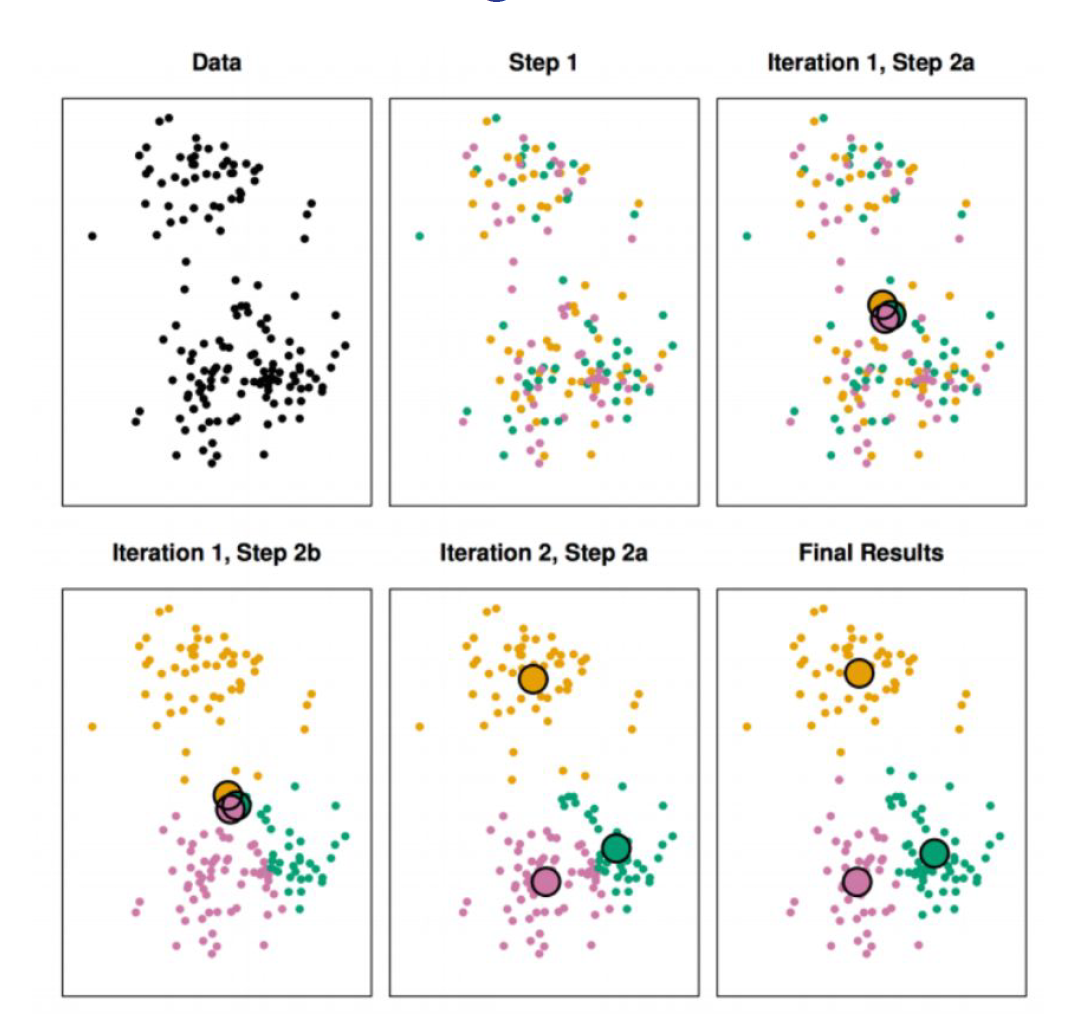
\includegraphics[width=0.45\linewidth ]{Figures/kmeans_algorithm.png}


\end{frame}
%----------------------------------------------------------------------------%

%----------------------------------------------------------------------------%

\begin{frame}
\frametitle{Choosing K}
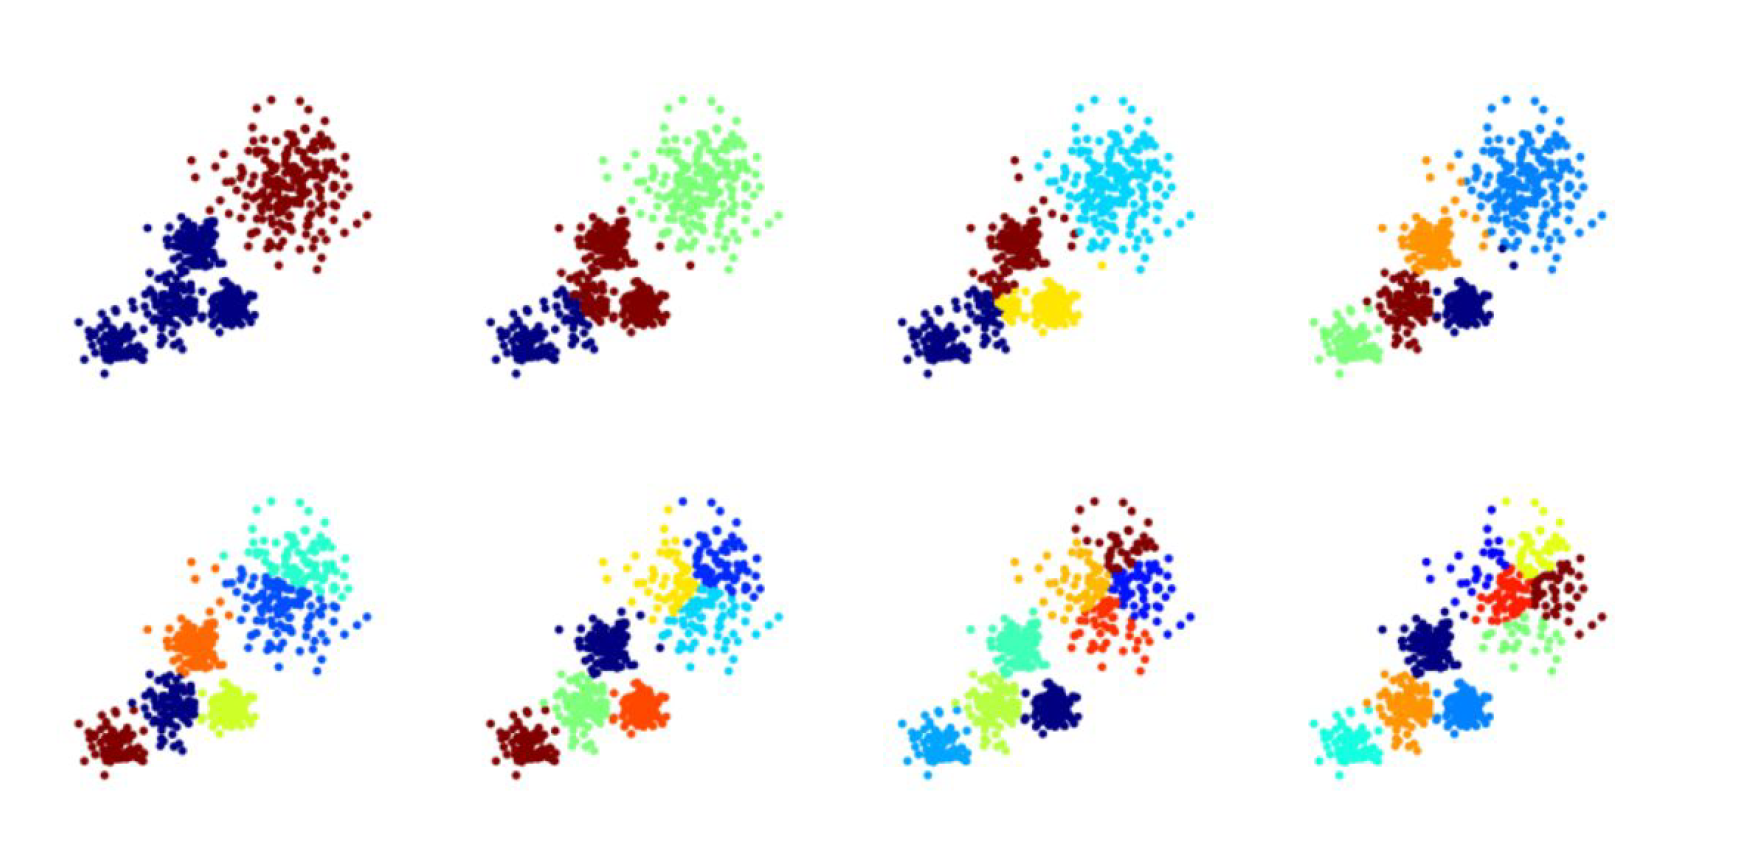
\includegraphics[width=0.85\linewidth ]{Figures/choosing_k.png}


\end{frame}
%----------------------------------------------------------------------------%

\begin{frame}
\frametitle{Choosing K}
There is no easy answer for choosing a "best" K value\\
One way is the elbow method\\
\begin{itemize}
\item First of all, compute the sum of squared error (SSE) for some
values of k (for example 2, 4, 6, 8, etc.)
\item The SSE is defined as the sum of the squared distance
between each member of the cluster and its centroid
\item If you plot k against the SSE, you will see that the error
decreases as k gets larger; this is because when the number
of clusters increases, they should be smaller, so distortion is
also smaller
\item The idea of the elbow method is to choose the k at which the
SSE decreases abruptly
\item This produces an "elbow effect" in the graph, as you can see
in the following picture:
\end{itemize}

\end{frame}
%----------------------------------------------------------------------------%
%----------------------------------------------------------------------------%

\begin{frame}
\frametitle{Elbow Method}
\centering 
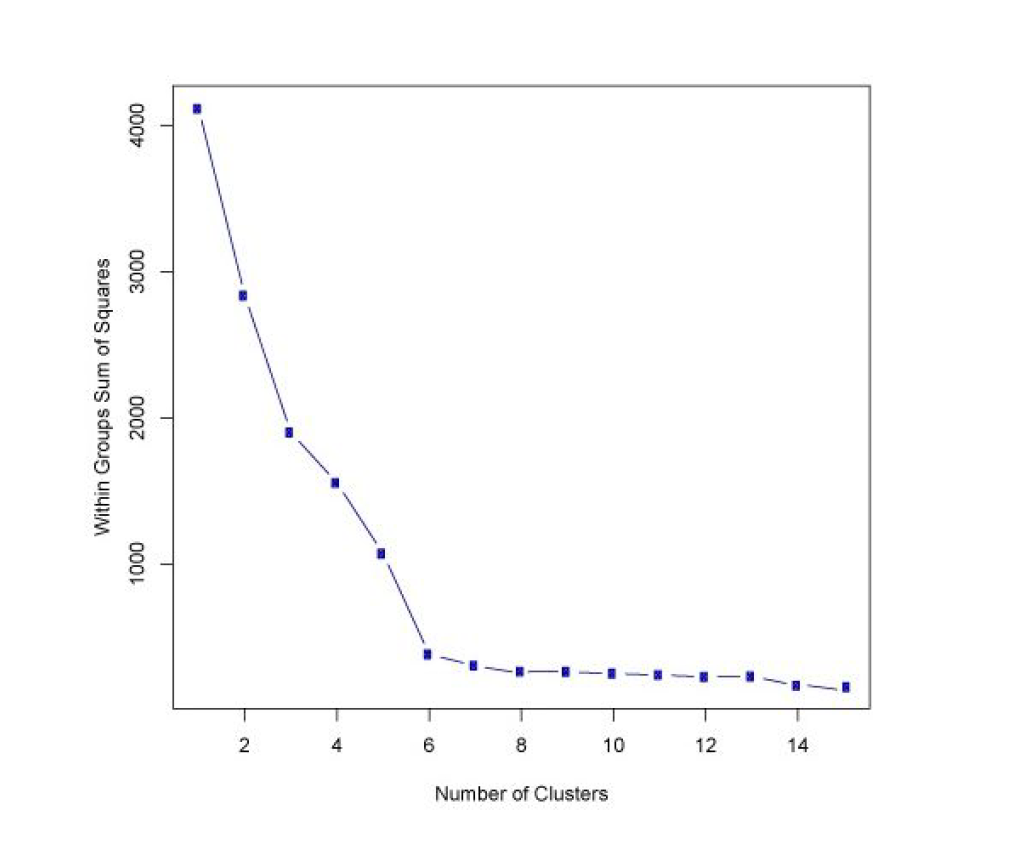
\includegraphics[width=0.65\linewidth ]{Figures/elbow_method.png}


\end{frame}
%----------------------------------------------------------------------------%


\end{document}





